% Provenance (never printed): BCPST year 1 geology (2021), "la carte
% geologique" (reading a map, structures, chronology), union licence
% Sciences de la Terre L1 (cartographie: strike and dip, three-point problem,
% outcrop patterns, DEM and GIS). See sources/outline_sources.md. Pilot
% chapter, 2026-10-22. The region is the series' invented Varden Hills
% (figdata/shared/region.py); every number about it is computed in
% figdata/bachelor-1/varden_maps.py or figdata/bachelor-1/v_rule.py.
\chapter{Les cartes géologiques}\label{ch:b1:geological-maps}

Un géologue traverse une chaîne de basses collines avec une planchette, un
carnet et une boussole à clinomètre. Presque partout, le sol est de l'herbe, du
bois ou un champ labouré~; la roche ne se montre qu'ici et là, dans la berge
d'un ruisseau, une tranchée de route, un rocher. À partir de ces aperçus
dispersés, et de la forme du terrain, le géologue doit dire quelle roche se
trouve sous chaque mètre carré des collines, comment les couches sont
inclinées, où elles sont rompues, et dans quel ordre tout cela s'est produit.
Le résultat est une \omterm{def:b1:geological-maps:geological-map}{carte géologique}~: un dessin plan qui code un corps de roche
à trois dimensions. Ce chapitre explique comment une telle carte se fait et se
lit --- comment l'\omterm{def:b1:geological-maps:attitude}{attitude} d'une surface se mesure et se calcule, pourquoi
l'\omterm{def:b1:geological-maps:geological-map}{affleurement} d'une couche dessine les figures qu'il dessine, et comment une
carte raconte une histoire. Ses exemples viennent d'une région imaginaire mais
géologiquement cohérente, les collines de Varden, qui reviennent tout au long de
ce livre.

\begin{recall}
Une carte topographique montre le relief par des courbes de niveau, lignes
d'égale altitude~; son échelle relie les distances sur la carte aux distances
sur le terrain (livre~1, année~9). Les âges relatifs découlent de la
superposition (une couche est plus jeune que celles qui sont dessous, à moins
que la série n'ait été renversée), du recoupement (ce qui recoupe une roche est
plus jeune qu'elle) et de l'inclusion (livre~1, année~7). Une faille est une
cassure le long de laquelle les deux blocs se sont déplacés (livre~1,
année~7)~; la géométrie des \omterm{def:b1:geological-maps:fold}{plis} et des failles fait l'objet du
\cref{ch:b1:faults-folds-fabrics}.
\end{recall}

\section{Une carte est une coupe à travers l'espace}\label{sec:b1:geological-maps:cut}

\begin{definition}[Carte géologique]\label{def:b1:geological-maps:geological-map}
Une \emph{carte géologique}\index{carte geologique@carte géologique} indique, en chaque point de la surface du
sol, l'unité rocheuse qui se trouve là sous le sol meuble, avec les
\emph{contacts}\index{contact (geologique)@contact (géologique)} --- surfaces séparant deux unités --- et les structures
(failles, axes de \omterm{def:b1:geological-maps:fold}{plis}, \omterm{def:b1:geological-maps:attitude}{attitudes} des couches) qui les affectent. Une
\emph{unité cartographique}\index{unite cartographique@unité cartographique} est un corps de roche que l'on peut reconnaître et
suivre sur le terrain et que l'on dessine d'une seule couleur~; son
\emph{affleurement}\index{affleurement} est la zone où elle se trouve à la
surface.
\end{definition}

\begin{definition}[Modèle numérique de terrain]\label{def:b1:geological-maps:dem}
Un \emph{modèle numérique de terrain}\index{modele numerique de terrain@modèle numérique de terrain} est une grille d'altitudes du
sol, $z = g(x,y)$, en des points régulièrement espacés. Un système
d'information géographique stocke de telles grilles et les autres couches de la
carte (\omterm{def:b1:geological-maps:geological-map}{contacts}, failles, mesures, sondages) dans un même repère de coordonnées
et calcule avec elles.
\end{definition}

\begin{proposition}[L'affleurement d'un contact]\label{prop:b1:geological-maps:intersection}
Soit le sol la surface $z = g(x,y)$ et un contact la surface
$z = c(x,y)$. La trace du contact sur la carte est la courbe
\[
  g(x,y) = c(x,y),
\]
projection sur le plan horizontal de l'intersection des deux surfaces. L'unité
située au-dessus du contact affleure là où $g > c$.
\end{proposition}

\begin{proof}
Un point de la carte se trouve sur la trace si et seulement si la surface du sol
en ce point appartient au contact, c'est-à-dire $g(x,y) = c(x,y)$. Là où
$g(x,y) > c(x,y)$, le sol est au-dessus du contact~: la roche en surface
appartient à l'unité située au-dessus.
\end{proof}

\begin{remark}[Comment les cartes de ce livre sont dessinées]\label{rem:b1:geological-maps:computed}
C'est exactement ainsi qu'un système d'information géographique dessine une
carte à partir d'un modèle tridimensionnel~: il évalue $g - c$ sur la grille
d'un \omterm{def:b1:geological-maps:dem}{modèle numérique de terrain} et trace les courbes où il change de signe. Les
cartes des collines de Varden de ce livre ont été dessinées de cette façon, à
partir d'un modèle géologique où chaque surface est connue.
\end{remark}

\begin{omfigure}
\begin{tikzpicture}
\begin{axis}[axis equal image, xmin=0, xmax=10, ymin=0, ymax=8, width=0.82\linewidth,
  tick label style={font=\scriptsize}, xlabel={est (km)}, ylabel={nord (km)},
  label style={font=\small}, colormap/blackwhite, enlargelimits=false]
\addplot[matrix plot*, mesh/cols=101, point meta=explicit, shader=interp] table[x=x_km, y=y_km, meta=shade] {figdata/out/bachelor-1-varden_maps-shade.dat};
\addplot[contour, line width=0.25pt, opacity=0.7] table {figdata/out/shared-region-contours.dat};
\addplot[index contour, opacity=0.8] table {figdata/out/shared-region-index-contours.dat};
\addplot[river] table {figdata/out/shared-region-river.dat};
\end{axis}
\end{tikzpicture}

{\small Les collines de Varden en \omterm{def:b1:geological-maps:dem}{modèle numérique de terrain}~: le sol éclairé
depuis le nord-ouest, avec des courbes de niveau tous les \qty{50}{m} (plus
épaisses à 250 et \qty{500}{m}) et la rivière, qui coule vers l'est.}
\end{omfigure}

\begin{omfigure}
\begin{tikzpicture}
\begin{axis}[axis equal image, xmin=0, xmax=10, ymin=0, ymax=8, width=0.82\linewidth,
  tick label style={font=\scriptsize}, xlabel={est (km)}, ylabel={nord (km)},
  label style={font=\small}]
\addplot[lith schist, draw=black, line width=0.3pt, even odd rule] table {figdata/out/shared-region-unit-schist.dat};
\addplot[lith granite, draw=black, line width=0.3pt, even odd rule] table {figdata/out/shared-region-unit-granite.dat};
\addplot[om lith={icsTriassic!35}{om sand}, draw=black, line width=0.3pt, even odd rule] table {figdata/out/shared-region-unit-sandstone.dat};
\addplot[om lith={icsJurassic!40}{om limestone}, draw=black, line width=0.3pt, even odd rule] table {figdata/out/shared-region-unit-limestone.dat};
\addplot[om lith={icsJurassic!15}{om shale}, draw=black, line width=0.3pt, even odd rule] table {figdata/out/shared-region-unit-shale.dat};
\addplot[om lith={icsCretaceous!35}{om limestone}, draw=black, line width=0.3pt, even odd rule] table {figdata/out/shared-region-unit-chalk.dat};
% the fault is drawn before the alluvium: the younger alluvial floor conceals it
\addplot[normal fault] table {figdata/out/shared-region-fault.dat};
\addplot[lith alluvium, draw=black, line width=0.3pt, even odd rule] table {figdata/out/shared-region-unit-alluvium.dat};
\addplot[contour, opacity=0.55] table {figdata/out/shared-region-contours.dat};
\addplot[river] table {figdata/out/shared-region-river.dat};
\pic at (axis cs:4.3,6.6) {strikedip={350.6}{12}};
\pic at (axis cs:2.2,6.6) {strikedip={189.3}{12}};
\pic at (axis cs:8.6,1.4) {northarrow};
\fill[black] (axis cs:6.6,0.35) rectangle (axis cs:7.1,0.5);
\fill[white] (axis cs:7.1,0.35) rectangle (axis cs:7.6,0.5);
\fill[black] (axis cs:7.6,0.35) rectangle (axis cs:8.1,0.5);
\fill[white] (axis cs:8.1,0.35) rectangle (axis cs:8.6,0.5);
\draw[black, line width=0.4pt] (axis cs:6.6,0.35) rectangle (axis cs:8.6,0.5);
\node[font=\footnotesize, above, inner sep=1.5pt, fill=white, fill opacity=0.8, text opacity=1] at (axis cs:7.6,0.5) {\qty{2}{km}};
\end{axis}
\end{tikzpicture}

\smallskip
\begin{tikzpicture}[font=\footnotesize]
\matrix[column sep=7pt, row sep=3pt, matrix of nodes, nodes={anchor=west}] {
  \tikz\draw[black!60, line width=0.4pt, lith alluvium] (0,0) rectangle (0.7,0.32); & alluvions (Quaternaire) &
  \tikz\draw[black!60, line width=0.4pt, om lith={icsCretaceous!35}{om limestone}] (0,0) rectangle (0.7,0.32); & craie (Crétacé, 90 Ma) \\
  \tikz\draw[black!60, line width=0.4pt, om lith={icsJurassic!15}{om shale}] (0,0) rectangle (0.7,0.32); & argilite (Jurassique, 165 Ma) &
  \tikz\draw[black!60, line width=0.4pt, om lith={icsJurassic!40}{om limestone}] (0,0) rectangle (0.7,0.32); & calcaire (Jurassique, 180 Ma) \\
  \tikz\draw[black!60, line width=0.4pt, om lith={icsTriassic!35}{om sand}] (0,0) rectangle (0.7,0.32); & grès (Trias, 245 Ma) &
  \tikz\draw[black!60, line width=0.4pt, lith granite] (0,0) rectangle (0.7,0.32); & granite (310 Ma) \\
  \tikz\draw[black!60, line width=0.4pt, lith schist] (0,0) rectangle (0.7,0.32); & schiste (480 Ma) &
  \tikz\draw[normal fault] (0,0.16) -- (0.9,0.16); & faille normale (traits sur le compartiment affaissé) \\
};
\end{tikzpicture}

{\small La \omterm{def:b1:geological-maps:geological-map}{carte géologique} des collines de Varden, avec les courbes de niveau,
la rivière, deux \omterm{def:b1:geological-maps:attitude}{attitudes} mesurées (trait de \omterm{def:b1:geological-maps:attitude}{direction} et tiret de \omterm{def:b1:geological-maps:attitude}{pendage},
avec le \omterm{def:b1:geological-maps:attitude}{pendage} en degrés) et la légende. Les âges sont ceux des unités de la
région~; la faille est cachée sous les alluvions plus récentes du fond de
vallée.}
\end{omfigure}

\section{L'attitude d'un plan}

\begin{definition}[Direction, pendage et sens du pendage]\label{def:b1:geological-maps:attitude}
Considérons une surface géologique --- plan de stratification, contact,
faille --- localement plane. Sa \emph{direction}\index{direction (d'un plan)} est celle des droites horizontales
qu'elle contient, donnée par un \omterm{def:b1:spherical-astronomy:horizontal}{azimut} (degrés dans le sens horaire à partir du
nord). Son \emph{pendage}\index{pendage} $\delta$ est l'angle entre le plan et
l'horizontale, mesuré dans le plan vertical perpendiculaire à la direction,
$0 \le \delta \le \ang{90}$. Son \emph{sens du pendage}\index{sens du pendage}
$\alpha$ est l'\omterm{def:b1:spherical-astronomy:horizontal}{azimut} de la ligne de plus grande pente du plan, orientée vers le
bas. Ensemble, ils forment l'\emph{attitude}\index{attitude (d'un plan)} du plan, écrite sens du
pendage/pendage, par exemple $080/12$.
\end{definition}

\begin{notation}[Direction par la règle de la main droite]\label{not:b1:geological-maps:rhr}
Une \omterm{def:b1:geological-maps:attitude}{direction} peut se lire dans deux sens opposés. La \emph{règle de la main
droite} retient celui pour lequel le plan plonge à droite d'un observateur qui
regarde le long de la \omterm{def:b1:geological-maps:attitude}{direction}~: \omterm{def:b1:geological-maps:attitude}{direction} $= \alpha - \ang{90}$ (modulo
\ang{360}). Sur une carte, le symbole est un trait de \omterm{def:b1:geological-maps:attitude}{direction} portant un
court tiret orienté vers le bas du \omterm{def:b1:geological-maps:attitude}{pendage}, accompagné de la valeur du \omterm{def:b1:geological-maps:attitude}{pendage}.
\end{notation}

\begin{omfigure}
\tdplotsetmaincoords{65}{125}
\begin{tikzpicture}[tdplot_main_coords, font=\small, scale=1.05]
  % the horizontal plane
  \fill[omSea!50] (-2.2,-1.6,0) -- (2.2,-1.6,0) -- (2.2,1.6,0) -- (-2.2,1.6,0) -- cycle;
  \draw[black!40] (-2.2,-1.6,0) -- (2.2,-1.6,0) -- (2.2,1.6,0) -- (-2.2,1.6,0) -- cycle;
  % the dipping plane: strike along y (north), dipping east (+x) at 30 degrees
  \fill[omLithLime!80, opacity=0.85] (-0.0,-1.6,0) -- (-0.0,1.6,0) -- (2.2,1.6,-1.27) -- (2.2,-1.6,-1.27) -- cycle;
  \draw[black!60] (0,-1.6,0) -- (0,1.6,0) -- (2.2,1.6,-1.27) -- (2.2,-1.6,-1.27) -- cycle;
  % strike line (horizontal, in both planes)
  \draw[omThm, line width=1.1pt] (0,-1.6,0) -- (0,1.6,0);
  % dip line and the horizontal below it, with the dip angle
  \draw[omDef, line width=1.1pt, -{Stealth[length=2.4mm]}] (0,0,0) -- (2.2,0,-1.27);
  \draw[black!60, densely dashed] (0,0,0) -- (2.2,0,0);
  \draw[black!60, densely dashed] (2.2,0,0) -- (2.2,0,-1.27);
  \draw[black] plot[domain=0:30, samples=16, variable=\t] ({0.8*cos(\t)}, 0, {-0.8*sin(\t)});
  \node[font=\footnotesize] at (1.05,0,-0.22) {$\delta$};
  % north arrow on the horizontal plane
  \draw[black, -{Stealth[length=2mm]}] (-1.8,-1.2,0) -- (-1.8,-0.3,0);
  \node[font=\footnotesize] at (-1.8,-0.05,0) {N};
\end{tikzpicture}
\begin{tikzpicture}[font=\small]
  \node[align=left, anchor=west, text width=5.2cm] at (0,0) {%
    \textcolor{omThm}{\rule[0.5ex]{0.6cm}{1.1pt}} direction~: une horizontale du plan~;\\[3pt]
    \textcolor{omDef}{\rule[0.5ex]{0.6cm}{1.1pt}} la ligne de plus grande pente du plan, dont l'azimut est le sens du pendage~;\\[3pt]
    le pendage est l'angle entre cette ligne et l'horizontale (en tirets).};
\end{tikzpicture}

{\small Un plan de \omterm{def:b1:geological-maps:attitude}{direction} nord et de \omterm{def:b1:geological-maps:attitude}{pendage} \ang{30} vers l'est (\omterm{def:b1:geological-maps:attitude}{attitude}
$090/30$), coupant un plan horizontal le long de sa ligne de \omterm{def:b1:geological-maps:attitude}{direction}. Hors
échelle.}
\end{omfigure}

\begin{proposition}[L'équation d'un plan incliné]\label{prop:b1:geological-maps:plane}
Avec $x$ vers l'est, $y$ vers le nord et $z$ vers le haut, le plan de \omterm{def:b1:geological-maps:attitude}{sens du
pendage} $\alpha$ et de \omterm{def:b1:geological-maps:attitude}{pendage} $\delta$ passant par le point $(x_0, y_0, z_0)$ est
\[
  z = z_0 - \tan\delta\,\bigl[(x - x_0)\sin\alpha + (y - y_0)\cos\alpha\bigr].
\]
\end{proposition}

\begin{proof}
Le vecteur unitaire horizontal dirigé selon le \omterm{def:b1:geological-maps:attitude}{sens du pendage} est
$\vec u = (\sin\alpha, \cos\alpha, 0)$ (un \omterm{def:b1:spherical-astronomy:horizontal}{azimut} se mesure à partir du nord,
l'axe $y$, vers l'est, l'axe $x$). Le long de la \omterm{def:b1:geological-maps:attitude}{direction}, perpendiculaire à
$\vec u$, le plan est horizontal~; le long de $\vec u$, il descend de
$\tan\delta$ par unité de distance horizontale. La distance horizontale d'un
point à la ligne de \omterm{def:b1:geological-maps:attitude}{direction} passant par $(x_0, y_0)$, comptée positivement
dans le \omterm{def:b1:geological-maps:attitude}{sens du pendage}, est $(x-x_0)\sin\alpha + (y-y_0)\cos\alpha$, d'où la
formule.
\end{proof}

\begin{theorem}[Attitude à partir de trois points]\label{thm:b1:geological-maps:three-point}
Soient $P_1, P_2, P_3$ trois points non alignés d'un plan, et
$\vec n = \overrightarrow{P_1P_2} \times \overrightarrow{P_1P_3} =
(n_x, n_y, n_z)$, choisi avec $n_z > 0$ (remplacer $\vec n$ par $-\vec n$
sinon). Alors le \omterm{def:b1:geological-maps:attitude}{pendage} et le \omterm{def:b1:geological-maps:attitude}{sens du pendage} du plan sont
\[
  \delta = \arccos\frac{n_z}{\|\vec n\|}, \qquad
  \alpha = \text{l'azimut du vecteur horizontal } (n_x, n_y),
\]
c'est-à-dire l'angle $\alpha \in [\ang{0}, \ang{360})$ tel que
$\sin\alpha = n_x/\sqrt{n_x^2+n_y^2}$ et $\cos\alpha = n_y/\sqrt{n_x^2+n_y^2}$
(le plan est horizontal si $n_x = n_y = 0$).
\end{theorem}

\begin{proof}
$\vec n$ est perpendiculaire à deux vecteurs indépendants du plan, donc normal à
celui-ci. Le \omterm{def:b1:geological-maps:attitude}{pendage} est l'angle entre le plan et l'horizontale, égal à l'angle
entre leurs normales, $\vec n$ et la verticale
$\vec k$~: $\cos\delta = \vec n \cdot \vec k / \|\vec n\| = n_z/\|\vec n\|$.
D'après la \cref{prop:b1:geological-maps:plane}, le plan est $z = \text{cste} -
\tan\delta\,(x\sin\alpha + y\cos\alpha)$, c'est-à-dire
$\tan\delta\sin\alpha\,x + \tan\delta\cos\alpha\,y + z = \text{cste}$~; sa
normale dirigée vers le haut est proportionnelle à $(\tan\delta\sin\alpha,
\tan\delta\cos\alpha, 1)$, dont la partie horizontale pointe dans le \omterm{def:b1:geological-maps:attitude}{sens du
pendage} $\alpha$. Comme $\vec n$ est un multiple positif de cette normale,
$(n_x, n_y)$ pointe lui aussi dans le \omterm{def:b1:geological-maps:attitude}{sens du pendage}.
\end{proof}

\begin{method}[Le problème des trois points]\label{met:b1:geological-maps:three-point}
Pour trouver l'\omterm{def:b1:geological-maps:attitude}{attitude} d'un contact rencontré dans trois sondages (ou vu à
trois \omterm{def:b1:geological-maps:geological-map}{affleurements})~:
\begin{enumerate}
  \item pour chaque sondage, prendre l'altitude du contact~: l'altitude du sol
        moins la profondeur à laquelle le contact a été rencontré~;
  \item écrire les trois points $P_i = (x_i, y_i, z_i)$ en mètres, $x$ vers
        l'est, $y$ vers le nord~;
  \item calculer $\vec n = \overrightarrow{P_1P_2} \times
        \overrightarrow{P_1P_3}$ et rendre $n_z$ positif~;
  \item appliquer le \cref{thm:b1:geological-maps:three-point}~; donner
        l'\omterm{def:b1:geological-maps:attitude}{attitude} sous la forme \omterm{def:b1:geological-maps:attitude}{sens du pendage}/\omterm{def:b1:geological-maps:attitude}{pendage} et, si on le demande,
        la \omterm{def:b1:geological-maps:attitude}{direction} par la règle de la main droite.
\end{enumerate}
Sur papier, le même problème se résout avec des isohypses structurales~: sur la
droite joignant le point le plus haut et le point le plus bas, trouver par
proportion le point situé à l'altitude du troisième~; la droite passant par ces
deux points de même altitude est une ligne de \omterm{def:b1:geological-maps:attitude}{direction}~; le \omterm{def:b1:geological-maps:attitude}{pendage} se déduit
de la différence d'altitude entre deux lignes de \omterm{def:b1:geological-maps:attitude}{direction} parallèles et de
leur écartement.
\end{method}

\begin{example}[Le flanc est de l'anticlinal de Varden]\label{ex:b1:geological-maps:east}
% computed in figdata/bachelor-1/varden_maps.py (boreholes E1-E3)
Trois sondages, E1 en $(4000, 6000)$, E2 en $(4600, 7200)$ et E3 en
$(5100, 6400)$ (mètres à l'est et au nord du coin sud-ouest de la carte),
rencontrent la base du calcaire aux altitudes $174$, $4$ et $\qty{-74}{m}$. Alors
$\overrightarrow{P_1P_2} = (600, 1200, -170)$,
$\overrightarrow{P_1P_3} = (1100, 400, -248)$~; leur produit vectoriel est
$(-229\,600, -38\,200, -1\,080\,000)$, qui pointe vers le bas, donc
\[
  \vec n = (229\,600,\ 38\,200,\ 1\,080\,000).
\]
Donc $\cos\delta = 1\,080\,000/\|\vec n\| \approx
0.9776$, $\delta \approx \ang{12.2}$, et le \omterm{def:b1:geological-maps:attitude}{sens du pendage} est l'\omterm{def:b1:spherical-astronomy:horizontal}{azimut} de
$(229\,600, 38\,200)$, $\alpha \approx \ang{80.6}$~: l'\omterm{def:b1:geological-maps:attitude}{attitude} est
$081/12$, \omterm{def:b1:geological-maps:attitude}{direction} $\ang{351}$ par la règle de la main droite. La base du
calcaire plonge doucement vers l'est-nord-est.
\end{example}

\section{Figures d'affleurement}

\begin{proposition}[Contacts horizontaux et verticaux]\label{prop:b1:geological-maps:hv}
La trace d'un contact horizontal suit la courbe de niveau de son altitude. La
trace d'un contact vertical est une droite sur la carte, quel que soit le
relief.
\end{proposition}

\begin{proof}
Pour $c(x,y) = z_0$, la trace $g(x,y) = z_0$ est la courbe de niveau $z_0$
(\cref{prop:b1:geological-maps:intersection}). Un plan vertical est l'ensemble
des points dont la position horizontale se trouve sur une même droite, à
n'importe quelle altitude~; sa trace sur la carte est cette droite.
\end{proof}

\begin{theorem}[La règle des V]\label{thm:b1:geological-maps:v-rule}
Un contact plan traverse une vallée dont le fond descend vers l'aval avec la
pente $s > 0$. Soit $a$ la tangente du \omterm{def:b1:geological-maps:attitude}{pendage} apparent du contact dans la
\omterm{def:b1:geological-maps:attitude}{direction} de l'aval ($a > 0$ s'il plonge vers l'aval, $a < 0$ s'il plonge vers
l'amont, $a = 0$ s'il est horizontal). Alors la trace de l'\omterm{def:b1:geological-maps:geological-map}{affleurement} dessine
un V dont le sommet se trouve sur le fond de la vallée et qui
\begin{itemize}
  \item pointe \emph{vers l'aval} si $a > s$~: le contact plonge vers l'aval
        plus fortement que ne descend le fond de la vallée~;
  \item pointe \emph{vers l'amont} si $a < s$~: le contact est horizontal,
        plonge vers l'amont, ou plonge vers l'aval moins fortement que le fond.
\end{itemize}
Un contact vertical ne dessine pas de V.
\end{theorem}

\begin{proof}
Soit $\xi$ la distance mesurée vers l'aval le long du fond de la vallée. Le
fond est à l'altitude $z_g(\xi) = z_0 - s\xi$~; dans la coupe verticale le long
de la vallée, le contact est à $z_c(\xi) = c - a\xi$. Sur le fond, la trace est
là où $z_g = z_c$~:
\[
  \xi_{\text{fond}} = \frac{c - z_0}{a - s}.
\]
Sur un versant, en un point plus haut que le fond de $h > 0$ et à la même
distance de la source de la vallée, le sol est à $z_0 - s\xi + h$, donc la trace
est là où $c - a\xi = z_0 - s\xi + h$~:
\[
  \xi_{\text{versant}} = \frac{c - z_0 - h}{a - s}, \qquad
  \xi_{\text{fond}} - \xi_{\text{versant}} = \frac{h}{a - s}.
\]
Si $a > s$, la trace se trouve plus loin vers l'aval sur le fond que sur les
versants~: le V pointe vers l'aval. Si $a < s$, c'est l'inverse. Un contact
vertical traverse le fond et les versants au même $\xi$.
\end{proof}

\begin{omfigure}
\begin{tikzpicture}
\pgfplotsset{vpanel/.style={axis equal image, xmin=-1, xmax=1, ymin=0, ymax=2,
  width=4.1cm, ticks=none, axis line style={black!50}, clip=true,
  title style={font=\footnotesize, align=center, yshift=-2pt}}}
\begin{axis}[vpanel, at={(0cm,0cm)}, title={horizontal}]
\addplot[contour, opacity=0.8] table {figdata/out/bachelor-1-v_rule-contours.dat};
\addplot[omThm, line width=1.2pt] table {figdata/out/bachelor-1-v_rule-h.dat};
\addplot[river, -{Stealth[length=1.6mm]}] coordinates {(0,0.05) (0,1.95)};
\end{axis}
\begin{axis}[vpanel, at={(3.15cm,0cm)}, title={plongeant\\vers l'amont}]
\addplot[contour, opacity=0.8] table {figdata/out/bachelor-1-v_rule-contours.dat};
\addplot[omThm, line width=1.2pt] table {figdata/out/bachelor-1-v_rule-u.dat};
\addplot[river, -{Stealth[length=1.6mm]}] coordinates {(0,0.05) (0,1.95)};
\end{axis}
\begin{axis}[vpanel, at={(6.3cm,0cm)}, title={vers l'aval,\\moins raide}]
\addplot[contour, opacity=0.8] table {figdata/out/bachelor-1-v_rule-contours.dat};
\addplot[omThm, line width=1.2pt] table {figdata/out/bachelor-1-v_rule-g.dat};
\addplot[river, -{Stealth[length=1.6mm]}] coordinates {(0,0.05) (0,1.95)};
\end{axis}
\begin{axis}[vpanel, at={(9.45cm,0cm)}, title={vers l'aval,\\plus raide}]
\addplot[contour, opacity=0.8] table {figdata/out/bachelor-1-v_rule-contours.dat};
\addplot[omThm, line width=1.2pt] table {figdata/out/bachelor-1-v_rule-d.dat};
\addplot[river, -{Stealth[length=1.6mm]}] coordinates {(0,0.05) (0,1.95)};
\end{axis}
\end{tikzpicture}

{\small La règle des V, calculée. Dans chaque panneau, une rivière (flèche
bleue) coule vers le nord dans une vallée, dont les courbes de niveau (tous les
\qty{10}{m}) pointent vers l'amont~; un contact de \omterm{def:b1:geological-maps:attitude}{direction} est--ouest est
tracé en rouge. Horizontal, il suit les courbes de niveau~; plongeant vers
l'amont, ou vers l'aval moins fortement que le fond de la vallée, il dessine un
V pointant vers l'amont~; plongeant vers l'aval plus fortement (ici \ang{10}),
un V pointant vers l'aval. Un contact vertical traverserait en ligne droite.}
\end{omfigure}

\begin{remark}[La largeur d'un affleurement]\label{rem:b1:geological-maps:width}
La largeur de l'\omterm{def:b1:geological-maps:geological-map}{affleurement} d'une unité dépend de son épaisseur, de son
\omterm{def:b1:geological-maps:attitude}{pendage} et de la pente du terrain~: une couche mince plongeant dans le même sens
que la pente peut affleurer sur une vaste surface. L'épaisseur se calcule à
partir d'une carte et d'une coupe au \cref{ch:b1:cross-sections}.
\end{remark}

\section{Plis, failles, intrusions et discordances sur une carte}

\begin{definition}[Anticlinal et synclinal]\label{def:b1:geological-maps:fold}
Un \emph{pli}\index{pli} est une courbure de couches initialement planes. Un
\emph{anticlinal}\index{anticlinal} est un pli dont les couches sont convexes
vers le haut (un pli en voûte)~; un \emph{synclinal}\index{synclinal} est un pli
dont les couches sont concaves vers le haut (un pli en creux). Les deux côtés
d'un pli sont ses flancs~; son \emph{axe du pli}\index{axe du pli} est la ligne le long de
laquelle les couches se courbent le plus, et l'axe plonge quand il n'est pas
horizontal. Une ligne telle qu'un axe de pli se repère par sa \omterm{def:b1:geological-maps:attitude}{direction},
l'\omterm{def:b1:spherical-astronomy:horizontal}{azimut} de sa projection horizontale pris vers le bas, et son plongement,
l'angle qu'elle fait avec l'horizontale (\cref{ch:b1:field-lab-methods-1}). La
géométrie des plis en trois dimensions fait l'objet du
\cref{ch:b1:faults-folds-fabrics}.
\end{definition}

\begin{proposition}[Les figures des plis]\label{prop:b1:geological-maps:folds}
Sur une carte de couches plissées et érodées, un \omterm{def:b1:geological-maps:fold}{anticlinal} montre les unités
les plus anciennes en son cœur et des unités plus jeunes vers l'extérieur de
part et d'autre~; un \omterm{def:b1:geological-maps:fold}{synclinal} montre les plus jeunes en son cœur. Si l'\omterm{def:b1:geological-maps:fold}{axe du
pli} plonge, les \omterm{def:b1:geological-maps:geological-map}{affleurements} se referment autour du \omterm{def:b1:geological-maps:fold}{pli}~: la fermeture d'un
\omterm{def:b1:geological-maps:fold}{anticlinal} pointe dans le sens du plongement, celle d'un \omterm{def:b1:geological-maps:fold}{synclinal} dans le sens
inverse.
\end{proposition}

\begin{proof}[Démonstration partielle]
Dans un \omterm{def:b1:geological-maps:fold}{anticlinal}, les couches montent vers l'axe, si bien qu'une surface
d'érosion à peu près plane entaille la série le plus profondément à cet endroit
et expose ses unités les plus anciennes, les plus basses~; dans un \omterm{def:b1:geological-maps:fold}{synclinal},
les unités les plus jeunes sont préservées le plus bas, au cœur. Si l'axe
plonge, considérons un contact d'un \omterm{def:b1:geological-maps:fold}{anticlinal}~: c'est une voûte dont la crête
descend le long du plongement. Là où la crête est au-dessus du sol, le sol coupe
la voûte le long de deux flancs~; là où la crête passe sous le sol, le contact
n'atteint plus la surface. Les deux flancs de la trace se rejoignent donc autour
du point où la crête rencontre le sol, et cette fermeture se trouve dans le sens
du plongement. Un \omterm{def:b1:geological-maps:fold}{synclinal} est une auge dont le fond remonte en sens inverse,
si bien que sa fermeture pointe contre le plongement. Le raisonnement suppose un
relief doux comparé à la descente de l'axe.
\end{proof}

\begin{proposition}[Failles, intrusions et discordances]\label{prop:b1:geological-maps:cuts}
Sur une carte~:
\begin{itemize}
  \item une faille interrompt et décale les \omterm{def:b1:geological-maps:geological-map}{contacts} qu'elle recoupe~; sur le
        bloc qui est descendu, des unités plus jeunes affleurent en face d'unités
        plus anciennes~; la trace d'une faille inclinée obéit à la règle des V
        comme n'importe quel plan~;
  \item un pluton ou un dyke recoupe les \omterm{def:b1:geological-maps:geological-map}{contacts} des roches dans lesquelles il
        s'injecte, et est plus jeune qu'elles~;
  \item à une discordance, les \omterm{def:b1:geological-maps:geological-map}{contacts} des roches plus anciennes sont tronqués
        le long de la base des plus jeunes, qui peuvent reposer successivement
        sur plusieurs unités plus anciennes.
\end{itemize}
\end{proposition}

\begin{method}[Lire l'histoire sur une carte]\label{met:b1:geological-maps:history}
\begin{enumerate}
  \item Lister les unités par ordre d'âge, d'après la légende et la
        superposition.
  \item Repérer ce qui recoupe quoi~: failles, intrusions, discordances~;
        chacune est plus jeune que tout ce qu'elle recoupe et plus ancienne que
        tout ce qui la scelle.
  \item Repérer les \omterm{def:b1:geological-maps:fold}{plis} et leurs axes~; un \omterm{def:b1:geological-maps:fold}{pli} est plus jeune que la plus jeune
        des unités qu'il plisse.
  \item Écrire les événements dans l'ordre, chacun avec l'indice présent sur la
        carte.
\end{enumerate}
\end{method}

\begin{example}[L'histoire des collines de Varden]\label{ex:b1:geological-maps:history}
Sur la carte des collines de Varden~: le schiste est l'unité la plus ancienne~;
le granite le recoupe, il est donc plus jeune~; le grès repose sur les deux en
tronquant le contour du granite~: une discordance, après une longue érosion. Le
grès, le calcaire, l'argilite et la craie se succèdent sans interruption et sont
plissés ensemble en un \omterm{def:b1:geological-maps:fold}{anticlinal} (grès et socle au cœur, près de
$x = \qty{3.5}{km}$) et un \omterm{def:b1:geological-maps:fold}{synclinal} (craie au cœur, à l'est du centre de la
carte)~: le plissement est postérieur au dépôt de la craie. La faille décale les
\omterm{def:b1:geological-maps:geological-map}{contacts} plissés~: elle est plus jeune que le plissement. Enfin la rivière s'est
enfoncée et a étalé ses alluvions, qu'aucune faille ne rompt.
\end{example}

\begin{inthefield}[Mesurer une attitude]
Sur une surface de stratification propre, le géologue pose l'arête d'une boussole
à clinomètre à l'horizontale et lit la \omterm{def:b1:geological-maps:attitude}{direction} sur la boussole, puis la pose
dans le sens de la plus grande pente et lit le \omterm{def:b1:geological-maps:attitude}{pendage} sur le clinomètre. Chaque
mesure est notée dans le carnet avec sa position et reportée aussitôt sur la
carte, de sorte qu'une lecture incohérente apparaisse alors que l'\omterm{def:b1:geological-maps:geological-map}{affleurement}
est encore sous la main. Aujourd'hui, les positions viennent de récepteurs
satellitaires, les mesures sont saisies sur des tablettes qui font tourner un
système d'information géographique, et les \omterm{def:b1:geological-maps:geological-map}{affleurements} sont photographiés et
placés sur des \omterm{def:b1:geological-maps:dem}{modèles numériques de terrain}.
\begin{center}
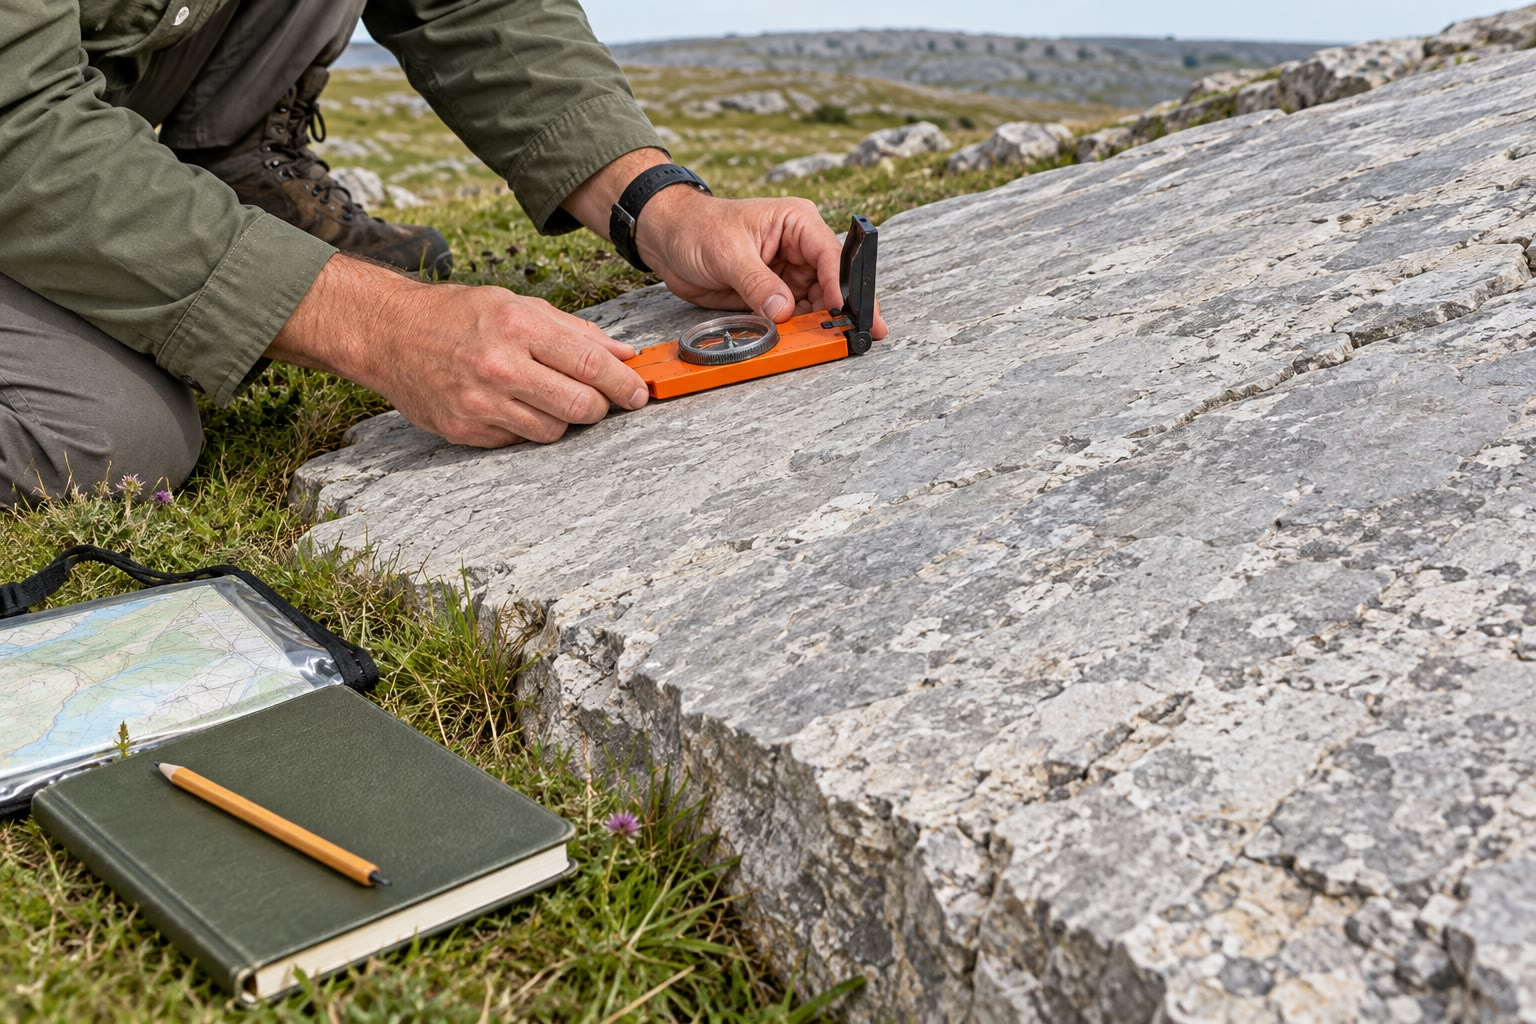
\includegraphics[width=0.6\linewidth]{images/book3/ai/b1-compass-clinometer.jpg}
\end{center}
\end{inthefield}

\begin{history}[La première carte géologique d'un pays]
% ledger: gsl:smith-1815, commons:smith-1815
L'arpenteur William Smith, qui creusait des canaux et drainait des terres en
Angleterre, remarqua que chaque couche de roche portait ses propres fossiles,
dans un ordre identique partout. Utilisant les fossiles pour reconnaître les
couches, il les suivit à travers le pays pendant plus de quinze ans. Sa carte,
intitulée \emph{A Delineation of the Strata of England and Wales, with part
of Scotland}, datée du 1\textsuperscript{er} août 1815, est considérée comme la
première \omterm{def:b1:geological-maps:geological-map}{carte géologique} d'un pays entier.
\begin{center}
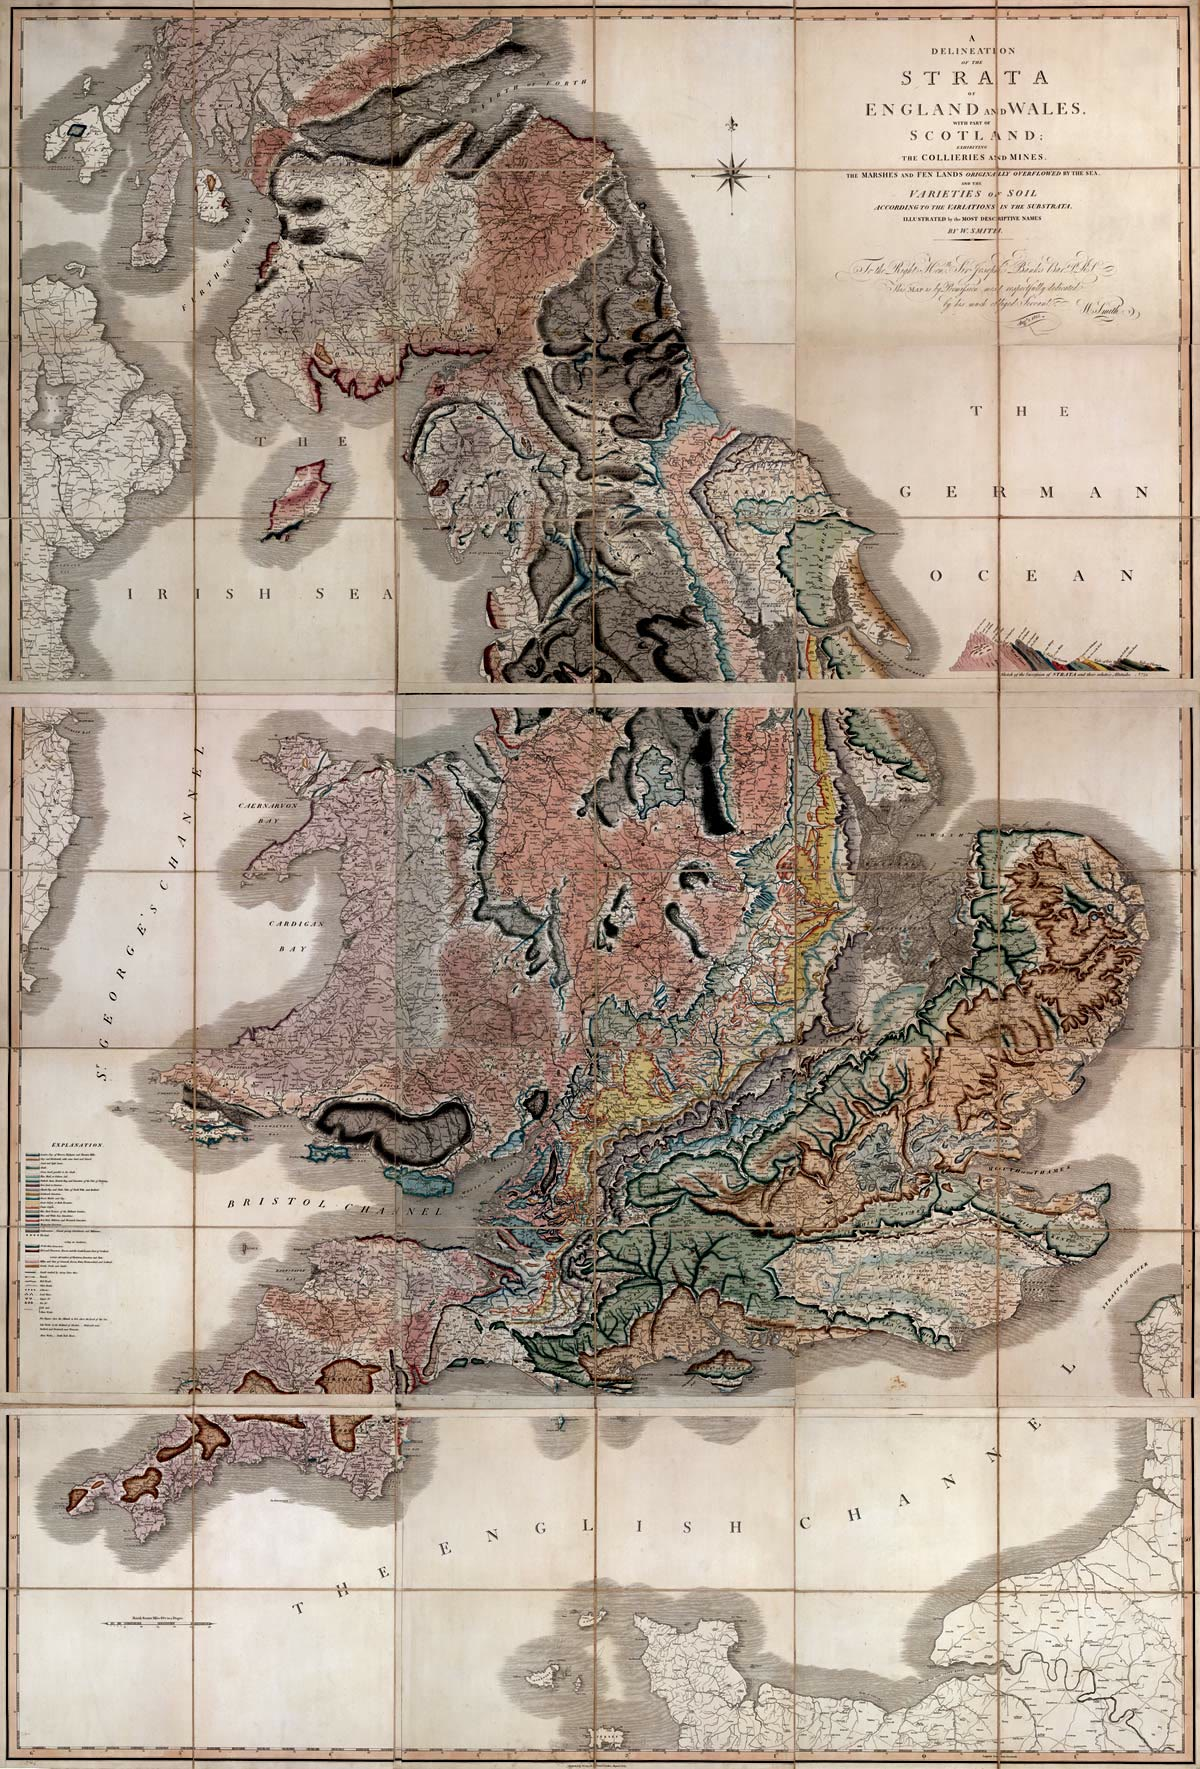
\includegraphics[width=0.36\linewidth]{images/book3/b1-smith-1815-map.jpg}

{\small La carte de William Smith de 1815 (domaine public).}
\end{center}
\end{history}

\section{Exercices}

\begin{exercise}[$\star$]\label{exo:b1:geological-maps:1}
Définir la \omterm{def:b1:geological-maps:attitude}{direction}, le \omterm{def:b1:geological-maps:attitude}{pendage} et le \omterm{def:b1:geological-maps:attitude}{sens du pendage} d'un plan. Une couche a
pour \omterm{def:b1:geological-maps:attitude}{attitude} $135/40$~: donner sa \omterm{def:b1:geological-maps:attitude}{direction} par la règle de la main droite et
dessiner son symbole cartographique.
\end{exercise}

\begin{exercise}[$\star$]\label{exo:b1:geological-maps:2}
Écrire l'équation du plan d'\omterm{def:b1:geological-maps:attitude}{attitude} $090/30$ passant par le point
$(0, 0, 500)$, coordonnées en mètres. À quelle altitude se trouve-t-il en
$(1000, 0)$ et en $(0, 1000)$~?
\end{exercise}

\begin{exercise}[$\star$]\label{exo:b1:geological-maps:3}
Sur une carte, la trace d'un contact suit exactement la courbe de niveau
\qty{350}{m}, sur plusieurs kilomètres de collines et de vallées. Que peut-on
dire de ce contact~? Et si sa trace est une droite à travers collines et
vallées~?
\end{exercise}

\begin{exercise}[$\star$]\label{exo:b1:geological-maps:4}
Sur la carte des collines de Varden, quelle unité affleure au cœur de
l'\omterm{def:b1:geological-maps:fold}{anticlinal} le long de la rivière, et quelle unité occupe le cœur du
\omterm{def:b1:geological-maps:fold}{synclinal}~? Expliquer pourquoi à l'aide du principe de superposition.
\end{exercise}

\begin{exercise}[$\star\star$]\label{exo:b1:geological-maps:5}
Un contact est rencontré aux altitudes $\qty{300}{m}$ en $(0, 0)$,
$\qty{300}{m}$ en $(1000, 0)$ et $\qty{200}{m}$ en $(0, 500)$ (mètres, $x$ vers
l'est, $y$ vers le nord). Trouver sa \omterm{def:b1:geological-maps:attitude}{direction}, son \omterm{def:b1:geological-maps:attitude}{sens du pendage} et son
\omterm{def:b1:geological-maps:attitude}{pendage}, d'abord par un raisonnement sur les isohypses structurales, puis avec
le \cref{thm:b1:geological-maps:three-point}.
\end{exercise}

\begin{exercise}[$\star\star$]\label{exo:b1:geological-maps:6}
Un fond de vallée descend vers le nord à \qty{30}{m} par km. De quel côté pointe
le V de l'\omterm{def:b1:geological-maps:geological-map}{affleurement} d'un contact si le contact (a) est horizontal~; (b)
plonge de \ang{20} vers le sud~; (c) plonge de \ang{1} vers le nord~; (d) plonge
de \ang{20} vers le nord~? Justifier avec le
\cref{thm:b1:geological-maps:v-rule}.
\end{exercise}

\begin{exercise}[$\star\star$]\label{exo:b1:geological-maps:7}
Dans la situation de la règle des V, un contact plonge vers l'aval avec
$a = 0.364$ (\ang{20}) et le fond de la vallée descend avec $s = 0.03$. Un point
du versant est à \qty{80}{m} au-dessus du fond. À quelle distance en amont du
sommet du V la trace se trouve-t-elle en ce point~?
\end{exercise}

\begin{exercise}[$\star\star$]\label{exo:b1:geological-maps:8}
Les \omterm{def:b1:geological-maps:geological-map}{affleurements} de l'\omterm{def:b1:geological-maps:fold}{anticlinal} de Varden se referment autour de l'extrémité
nord de son cœur. Dans quelle \omterm{def:b1:geological-maps:attitude}{direction} l'\omterm{def:b1:geological-maps:fold}{axe du pli} plonge-t-il~? Les
\omterm{def:b1:geological-maps:geological-map}{affleurements} du \omterm{def:b1:geological-maps:fold}{synclinal} se refermeraient-ils au nord ou au sud~?
\end{exercise}

\begin{exercise}[$\star\star$]\label{exo:b1:geological-maps:9}
Sur la \omterm{def:b1:geological-maps:geological-map}{carte géologique}, le long de la faille, quel côté montre en surface des
unités plus jeunes~? Quel bloc est descendu~? Vérifier avec le symbole de la carte.
\end{exercise}

\begin{exercise}[$\star\star\star$]\label{exo:b1:geological-maps:10}
Montrer que deux plans d'\omterm{def:b1:geological-maps:attitude}{attitudes} $(\alpha_1, \delta_1)$ et
$(\alpha_2, \delta_2)$ se coupent suivant une droite parallèle à
$\vec n_1 \times \vec n_2$, où $\vec n_i = (\tan\delta_i\sin\alpha_i,
\tan\delta_i\cos\alpha_i, 1)$. L'appliquer aux plans $090/30$ et $270/30$~:
quelle est cette droite, et quelle sorte de \omterm{def:b1:geological-maps:fold}{pli} forment les deux plans~?
\end{exercise}

\begin{exercise}[$\star\star\star$]\label{exo:b1:geological-maps:11}
Un dyke vertical de \omterm{def:b1:geological-maps:attitude}{direction} \ang{045} affleure à l'origine, sur un fond de
vallée à l'altitude \qty{0}{m}. Où peut se trouver sa trace sur une colline à
\qty{300}{m}~? Un second dyke a la même \omterm{def:b1:geological-maps:attitude}{direction}, plonge de \ang{60} vers le
sud-est et affleure lui aussi à l'origine. À quelle distance de l'origine, et
dans quelle \omterm{def:b1:geological-maps:attitude}{direction}, se trouve sa trace sur un terrain à \qty{300}{m},
mesurée perpendiculairement à la \omterm{def:b1:geological-maps:attitude}{direction}~?
\end{exercise}

\begin{exercise}[$\star\star\star$]\label{exo:b1:geological-maps:12}
Dans un \omterm{def:b1:geological-maps:dem}{modèle numérique de terrain} à maille de \qty{100}{m}, le sol en
$(x, y)$ et en $(x + 100, y)$ est à 420 et \qty{405}{m}, et en
$(x, y + 100)$ à \qty{412}{m}. En traitant le sol de cette maille comme un plan,
calculer sa pente (en degrés) et l'\omterm{def:b1:spherical-astronomy:horizontal}{azimut} vers lequel il est tourné (sens de la
plus grande pente).
\end{exercise}

\section{Problème~: Résoudre les collines de Varden}

\begin{problem}[{Problème du week-end --- des sondages et d'une carte à l'axe du
pli, à la faille et à l'histoire d'une région}]
\label{pb:b1:geological-maps:1}
% all data computed in figdata/bachelor-1/varden_maps.py from the region's
% model (figdata/shared/region.py); invented region: exercise data, no ledger
Une société qui fore pour chercher de l'eau dans les collines de Varden relève
les profondeurs où ses sondages rencontrent la base du calcaire~; ses géologues
repèrent aussi la faille là où elle traverse le sol. Les coordonnées sont en
mètres à l'est et au nord du coin sud-ouest de la carte~; les altitudes, en
mètres au-dessus du niveau de la mer. La partie I utilise la \omterm{def:b1:geological-maps:geological-map}{carte géologique} en
couleurs de la \cref{sec:b1:geological-maps:cut}.

\medskip
\noindent\textbf{Partie I --- Lire la carte.}
\begin{enumerate}
  \item Lister les unités de la région de la plus ancienne à la plus jeune.
  \item Quelles unités la rivière traverse-t-elle, d'ouest en est~?
  \item Quelle unité occupe le cœur du \omterm{def:b1:geological-maps:fold}{pli} près de $x = \qty{3.5}{km}$~? De
        quelle sorte de \omterm{def:b1:geological-maps:fold}{pli} s'agit-il~?
  \item Quelle unité occupe le cœur du \omterm{def:b1:geological-maps:fold}{pli} près de $x = \qty{7.5}{km}$~? De
        quelle sorte de \omterm{def:b1:geological-maps:fold}{pli} s'agit-il~?
  \item Pourquoi le schiste et le granite ne sont-ils visibles que près de la
        rivière, au cœur du premier \omterm{def:b1:geological-maps:fold}{pli}~?
  \item Quelle sorte de contact sépare le grès du granite~? Justifier d'après la
        carte.
\end{enumerate}

\medskip
\noindent Les sondages (profondeur $d$ jusqu'à la base du calcaire, altitude du
sol $z_g$) et les trois points F1--F3 où la faille traverse le toit du substrat
rocheux (F2, dans la vallée, se trouve sous les minces alluvions, que la faille
ne recoupe pas)~:

\begin{omfigure}
\begin{minipage}[c]{0.42\linewidth}
\centering\small
\begin{tabular}{lrrrr}
\hline
 & est & nord & $z_g$ & $d$ \\
\hline
E1 & 4000 & 6000 & 435 & 261 \\
E2 & 4600 & 7200 & 432 & 428 \\
E3 & 5100 & 6400 & 512 & 586 \\
W1 & 1500 & 6000 & 524 & 669 \\
W2 & 2200 & 7200 & 421 & 459 \\
W3 & 2600 & 5400 & 319 & 209 \\
\hline
 & est & nord & $z_g$ & \\
\hline
F1 & 4197 & 1000 & 405 & \\
F2 & 5824 & 3500 & 129 & \\
F3 & 7321 & 6500 & 482 & \\
\hline
\end{tabular}
\end{minipage}\hfill
\begin{minipage}[c]{0.56\linewidth}
\centering
\begin{tikzpicture}
\begin{axis}[axis equal image, xmin=0, xmax=10, ymin=0, ymax=8, width=\linewidth,
  tick label style={font=\scriptsize}, xlabel={est (km)}, ylabel={nord (km)},
  label style={font=\footnotesize}]
\addplot[fill=black!8, draw=black!50, line width=0.3pt, even odd rule] table {figdata/out/shared-region-unit-schist.dat};
\addplot[fill=black!8, draw=black!50, line width=0.3pt, even odd rule] table {figdata/out/shared-region-unit-granite.dat};
\addplot[fill=icsTriassic!20, draw=black!50, line width=0.3pt, even odd rule] table {figdata/out/shared-region-unit-sandstone.dat};
\addplot[fill=icsJurassic!25, draw=black!50, line width=0.3pt, even odd rule] table {figdata/out/shared-region-unit-limestone.dat};
\addplot[fill=icsJurassic!8, draw=black!50, line width=0.3pt, even odd rule] table {figdata/out/shared-region-unit-shale.dat};
\addplot[fill=icsCretaceous!20, draw=black!50, line width=0.3pt, even odd rule] table {figdata/out/shared-region-unit-chalk.dat};
\addplot[fault] table {figdata/out/shared-region-fault.dat};
\addplot[fill=omLithAlluv, draw=black!50, line width=0.3pt, even odd rule] table {figdata/out/shared-region-unit-alluvium.dat};
\addplot[river] table {figdata/out/shared-region-river.dat};
\addplot[only marks, mark=*, mark size=1.6pt] table[x=x_km, y=y_km] {figdata/out/bachelor-1-varden_maps-boreholes.dat};
\addplot[only marks, mark=square*, mark size=1.5pt, omThm] table[x=x_km, y=y_km] {figdata/out/bachelor-1-varden_maps-fault.dat};
\begin{scope}[every node/.style={font=\scriptsize\bfseries, inner sep=1.5pt, fill=white, fill opacity=0.8, text opacity=1}]
  \node[above right] at (axis cs:4,6) {E1};
  \node[above] at (axis cs:4.6,7.2) {E2};
  \node[right] at (axis cs:5.1,6.4) {E3};
  \node[above left] at (axis cs:1.5,6) {W1};
  \node[above] at (axis cs:2.2,7.2) {W2};
  \node[left] at (axis cs:2.6,5.4) {W3};
  \node[left, text=omThm] at (axis cs:4.197,1) {F1};
  \node[left, text=omThm] at (axis cs:5.824,3.5) {F2};
  \node[left, text=omThm] at (axis cs:7.321,6.5) {F3};
\end{scope}
\end{axis}
\end{tikzpicture}
\end{minipage}
\end{omfigure}

\medskip
\noindent\textbf{Partie II --- Le flanc est.}
\begin{enumerate}[resume]
  \item Calculer l'altitude de la base du calcaire en E1, E2 et E3.
  \item Écrire les vecteurs $\overrightarrow{E_1E_2}$ et
        $\overrightarrow{E_1E_3}$.
  \item Calculer leur produit vectoriel et l'orienter vers le haut.
  \item En déduire le \omterm{def:b1:geological-maps:attitude}{pendage} de la base du calcaire sur le flanc est.
  \item En déduire son \omterm{def:b1:geological-maps:attitude}{sens du pendage}, puis sa \omterm{def:b1:geological-maps:attitude}{direction} par la règle de la
        main droite.
  \item Le résultat est-il cohérent avec le symbole de \omterm{def:b1:geological-maps:attitude}{direction} et de \omterm{def:b1:geological-maps:attitude}{pendage}
        du flanc est sur la carte~?
\end{enumerate}

\medskip
\noindent\textbf{Partie III --- Le pli.}
\begin{enumerate}[resume]
  \item Calculer les altitudes de la base du calcaire en W1, W2 et
        W3.
  \item Calculer une normale $\vec n_W$ dirigée vers le haut à la base du
        calcaire sur le flanc ouest.
  \item En déduire l'\omterm{def:b1:geological-maps:attitude}{attitude} du flanc ouest.
  \item Calculer une \omterm{def:b1:geological-maps:attitude}{direction} de l'intersection des deux flancs, l'\omterm{def:b1:geological-maps:fold}{axe du pli},
        comme $\vec n_E \times \vec n_W$ (avec $\vec n_E$ issu de la question 9).
  \item Donner la \omterm{def:b1:geological-maps:attitude}{direction} (l'\omterm{def:b1:spherical-astronomy:horizontal}{azimut} de la projection horizontale de l'axe, pris
        vers le bas) et le plongement (son angle sous l'horizontale) de l'\omterm{def:b1:geological-maps:fold}{axe du
        pli}.
  \item La base du grès se trouve sur l'axe à \qty{230}{m} là où la rivière le
        traverse, près de $y = \qty{4}{km}$. De combien est-elle plus basse sur
        l'axe \qty{8}{km} plus au nord~? Est-ce cohérent avec la question 3 de
        la partie I et avec la fermeture des \omterm{def:b1:geological-maps:geological-map}{affleurements}~?
\end{enumerate}

\medskip
\noindent\textbf{Partie IV --- La faille et l'histoire.}
\begin{enumerate}[resume]
  \item À partir de F1, F2 et F3, calculer l'\omterm{def:b1:geological-maps:attitude}{attitude} de la faille.
  \item Le long de la faille, les unités affleurant du côté est-sud-est sont plus
        jeunes que celles qui leur font face. Quel bloc est descendu~? La faille
        est-elle normale ou inverse~?
  \item La droite de F1 à F3 passe à environ \qty{200}{m} à l'ouest de F2.
        Pourquoi la trace de la faille s'infléchit-elle vers l'est-sud-est là où
        elle traverse la vallée de la rivière, en F2~?
  \item Mettre dans l'ordre~: plissement~; dépôt de la craie~; jeu de la faille~;
        intrusion du granite~; érosion avant le grès~; dépôt des alluvions.
  \item La craie a 90 millions d'années et est plissée~; les alluvions se sont
        déposées au cours des 2.58 derniers millions d'années et ne sont pas
        faillées. Entre quels âges se sont produits le plissement et le jeu de la
        faille~?
  \item Pour atteindre la faille à \qty{1000}{m} sous le niveau de la mer sous
        F1, à quelle distance de F1, et dans quelle \omterm{def:b1:geological-maps:attitude}{direction}, faut-il forer un
        puits vertical~?
\end{enumerate}
\end{problem}
